\section{Actividad No 02 – Reconociendo la estructura} 

\begin{enumerate}[1.]
	\item Se requiere determinar la estructura de la tabla DEPARTMENTS y sus datos.

\begin{itemize}
	\begin{center}
	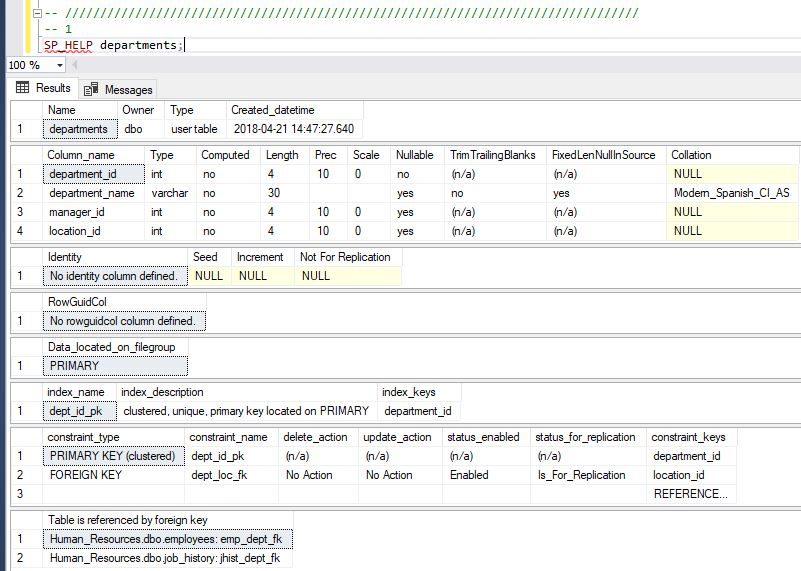
\includegraphics[width=5cm]{./Imagenes/actividad0201} 
	\end{center}
\end{itemize}

	\item El departamento de Recursos Humanos requiere un reporte que muestre los campos: employee\_id, last\_name y job\_id, asicomo el campo hire\_date con el alias StartDate.

\begin{itemize}
	\begin{center}
	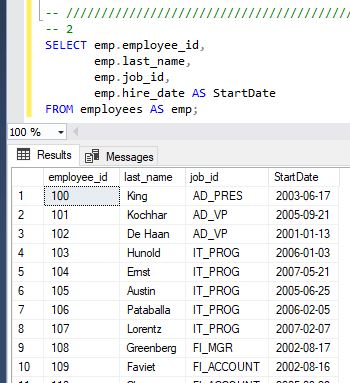
\includegraphics[width=5cm]{./Imagenes/actividad0202} 
	\end{center}
\end{itemize}

	\item Finalmente el departamento de Recursos Humanos requiere un listado de todos valores del campo JOB\_ID de la tabla EMPLOYEES pero que se muestren de forma única y no repetida.
\end{enumerate}

\begin{itemize}
	\begin{center}
	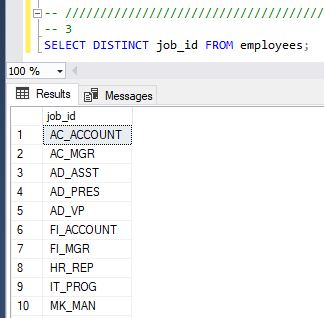
\includegraphics[width=5cm]{./Imagenes/actividad0203} 
	\end{center}
\end{itemize}

